% geometry_and_trigonometry:x01 GDC:NO
\begin{question}
  \hspace*{\fill} [Note Maximale: 7]\par
  \begin{center} % or flushleft or flushright
    \noindent Cercle de centre $O$ et de rayon égale à $r$ cm.\par
    \noindent La figure nest pas à l'échelle.\par
    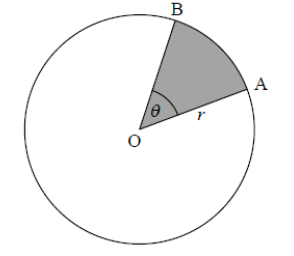
\includegraphics[scale=0.4]{figure_x1}\par

  \end{center} % or flushleft or flushright

  \noindent Les points $A$ et $B$ sont situés sur la circonférence du cercle et $\angle AOB = \theta$. L'aire du secteur grisé $AOB$ est de $12 cm^2$ et la longueur de l'arc $AB$ est de $6 cm$.\par
  \medskip
   \noindent Trouvez la valeur de $r$.\hspace*{\fill} [?]\par
\end{question}
